\section{\texorpdfstring{Mixed Binning: $P_t$ vs.~$z$}{New kinematic Bins: pt Vs z bin}}
\label{sec:newbins}
To better understand the kinematic dependence of Collins fragmentation, a new mixed binning in $z$ and $P_t$ is introduced in this section. For each $P_t$ bin, 4 different $z$ bins are used. This binning explores the kinematic dependence of the Collins FF more completely, since it is expected that $H_1^{\bot}$ depends non-trivially on both $z$ and $P_t$ without factorizing. 
As  for the other binning choices explored, the background correction has only a small effect on the asymmetry. 
The thrust-smearing correction is calculated the same way as in the Section~\ref{sec:smearingcorrection}. 
Table~\ref{tab:16binsthrustfactor_compare} shows the resulting smearing-correction factors and Table~\ref{tab:zptcharmratio} shows the charm ratios. 
Notice that the fourth bin is empty because no hadron in the lowest $z$ bin populates the highest $P_t$ bin. 
Figure~\ref{fig:ptznocorrection} shows the raw asymmetries, e.g., without any correction. For Fig.~\ref{fig:ptzbkgcorrection} the background correction has been applied, while Fig.~\ref{fig:ptzallcorrection} shows the results after background and thrust-smearing corrections. 

\begin{table}[H]\tiny
\centering
\begin{tabular}{|c|c|c|}
\hline
$P_{t1}$ [GeV]  & $z_{1}$  & correction factors   \\ \hline\hline
[0,0.15] & [0.2,0.3]	&		1.28	\\ \hline
[0.15,0.3] & [0.2,0.3] 	&		1.19	\\ \hline
[0.3,0.5]  & [0.2,0.3] 	&		1.13	\\ \hline
[0.5,3] & [0.2,0.3]  	&				\\ \hline\hline
[0,0.15] & [0.3,0.5]	&		1.62	\\ \hline
[0.15,0.3] & [0.3,0.5] 	&		1.28	\\ \hline
[0.3,0.5] & [0.3,0.5] 	&		1.17	\\ \hline
[0.5,3.0] & [0.3,0.5] 	&		1.29	\\ \hline\hline
[0,0.15] & [0.5,0.7] 	&		1.41	\\ \hline
[0.15,0.3] & [0.5,0.7] 	&		1.13	\\ \hline
[0.3,0.5] & [0.5,0.7]  	&		1.00	\\ \hline
[0.5,3.0] & [0.5,0.7]  	&		1.00	\\ \hline\hline
[0,0.15] & [0.7,1.0]	&		2.10	\\ \hline
[0.15,0.5]   & [0.7,1.0] 	&		1.37	\\ \hline
[0.3,0.5]  & [0.7,1.0] 	&		1.16	\\ \hline
[0.5,3.0] & [0.7,1.0]	&		1.08	\\ \hline
\end{tabular}
\caption{Thrust correction factors for $\pi^0$ $(z_1,P_{t1})$ bins.}
\label{tab:16binsthrustfactor_compare}
\end{table}


%\begin{table}[H]\footnotesize
%\centering
%\begin{tabular}{|l|l|l|l|l|}
%\hline
%$P_{t1}$  & $z_{1}$ &  $\pi^0$ simulated  & $\pi^0$ directly measure   \\ \hline
%[0,0.15] & [0.1,0.3]	&	1.38	&	1.28	\\ \hline
%[0.15,0.3] & [0.1,0.3] 	&	1.26	&	1.19	\\ \hline
%[0.3,0.5]  & [0.1,0.3] 	&	1.20	&	1.13	\\ \hline
%[0.5,3] & [0.1,0.3]  	&		&		\\ \hline
%[0,0.15] & [0.3,0.5]	&	1.67	&	1.62	\\ \hline
%[0.15,0.3] & [0.3,0.5] 	&	1.43	&	1.28	\\ \hline
%[0.3,0.5] & [0.3,0.5] 	&	1.34	&	1.17	\\ \hline
%[0.5,3.0] & [0.3,0.5] 	&	1.22	&	1.29	\\ \hline
%[0,0.15] & [0.5,0.7] 	&	2.12	&	1.41	\\ \hline
%[0.15,0.3] & [0.5,0.7] 	&	1.68	&	1.13	\\ \hline
%[0.3,0.5] & [0.5,0.7]  	&	1.54	&	1.00	\\ \hline
%[0.5,3.0] & [0.5,0.7]  	&	1.28	&	1.00	\\ \hline
%[0,0.15] & [0.7,1.0]	&	2.30	&	2.10	\\ \hline
%[0.15,0.5]   & [0.7,1.0] 	&	1.70	&	1.37	\\ \hline
%[0.3,0.5]  & [0.7,1.0] 	&	1.57	&	1.16	\\ \hline
%[0.5,3.0] & [0.7,1.0]	&	1.42	&	1.08	\\ \hline
%\end{tabular}
%\caption{Thrust correction factors for $\pi^0$ and $\eta$ $(z_1,z_2)$ bins.}
%\label{tab:16binsthrustfactor_compare}
%\end{table}
\begin{table}[H]\tiny
\centering
\begin{tabular}{|c|c|c|c|}
\hline
$z_1$ & $P_{t1}$ [GeV] &$\pi^{\pm}\pi^{\pm}$ & $\pi^{\pm}\pi^0$ \\ \hline\hline
[0.2,0.3]	&	[0,0.15]	&	22.85	&	24.63	\\ \hline
[0.2,0.3]	&	[0.15,0.30]	&	22.40	&	24.08	\\ \hline
[0.2,0.3]	&	[0.30,0.50]	&	21.88	&	22.98	\\ \hline
[0.2,0.3]	&	[0.50,3.0]	&		&		\\ \hline\hline
[0.3,0.5]	&	[0,0.15]	&	16.13	&	16.55	\\ \hline
[0.3,0.5]	&	[0.15,0.30]	&	16.46	&	16.85	\\ \hline
[0.3,0.5]	&	[0.30,0.50]	&	17.94	&	18.07	\\ \hline
[0.3,0.5]	&	[0.50,3.0]	&	20.79	&	20.38	\\ \hline\hline
[0.5,0.7]	&	[0,0.15]	&	10.54	&	15.78	\\ \hline
[0.5,0.7]	&	[0.15,0.30]	&	10.97	&	16.05	\\ \hline
[0.5,0.7]	&	[0.30,0.50]	&	12.53	&	17.27	\\ \hline
[0.5,0.7]	&	[0.50,3.0]	&	15.78	&	18.54	\\ \hline\hline
[0.7,1.0]	&	[0,0.15]	&	3.37	&	9.53	\\ \hline
[0.7,1.0]	&	[0.15,0.30]	&	3.96	&	10.01	\\ \hline
[0.7,1.0]	&	[0.30,0.50]	&	4.68	&	11.34	\\ \hline
[0.7,1.0]	&	[0.50,3.0]	&	6.42	&	13.75	\\ \hline
\end{tabular}
\caption[Charm ratio in $(z_{1},P_{t1})$ bins]{Charm ratio in $(z_{1},P_{t1})$ bins. All numbers are in percent.}
\label{tab:zptcharmratio}
\end{table}

\begin{figure}[t]
 \centering     \tiny
  \subfigure[No correction]{\label{fig:ptznocorrection}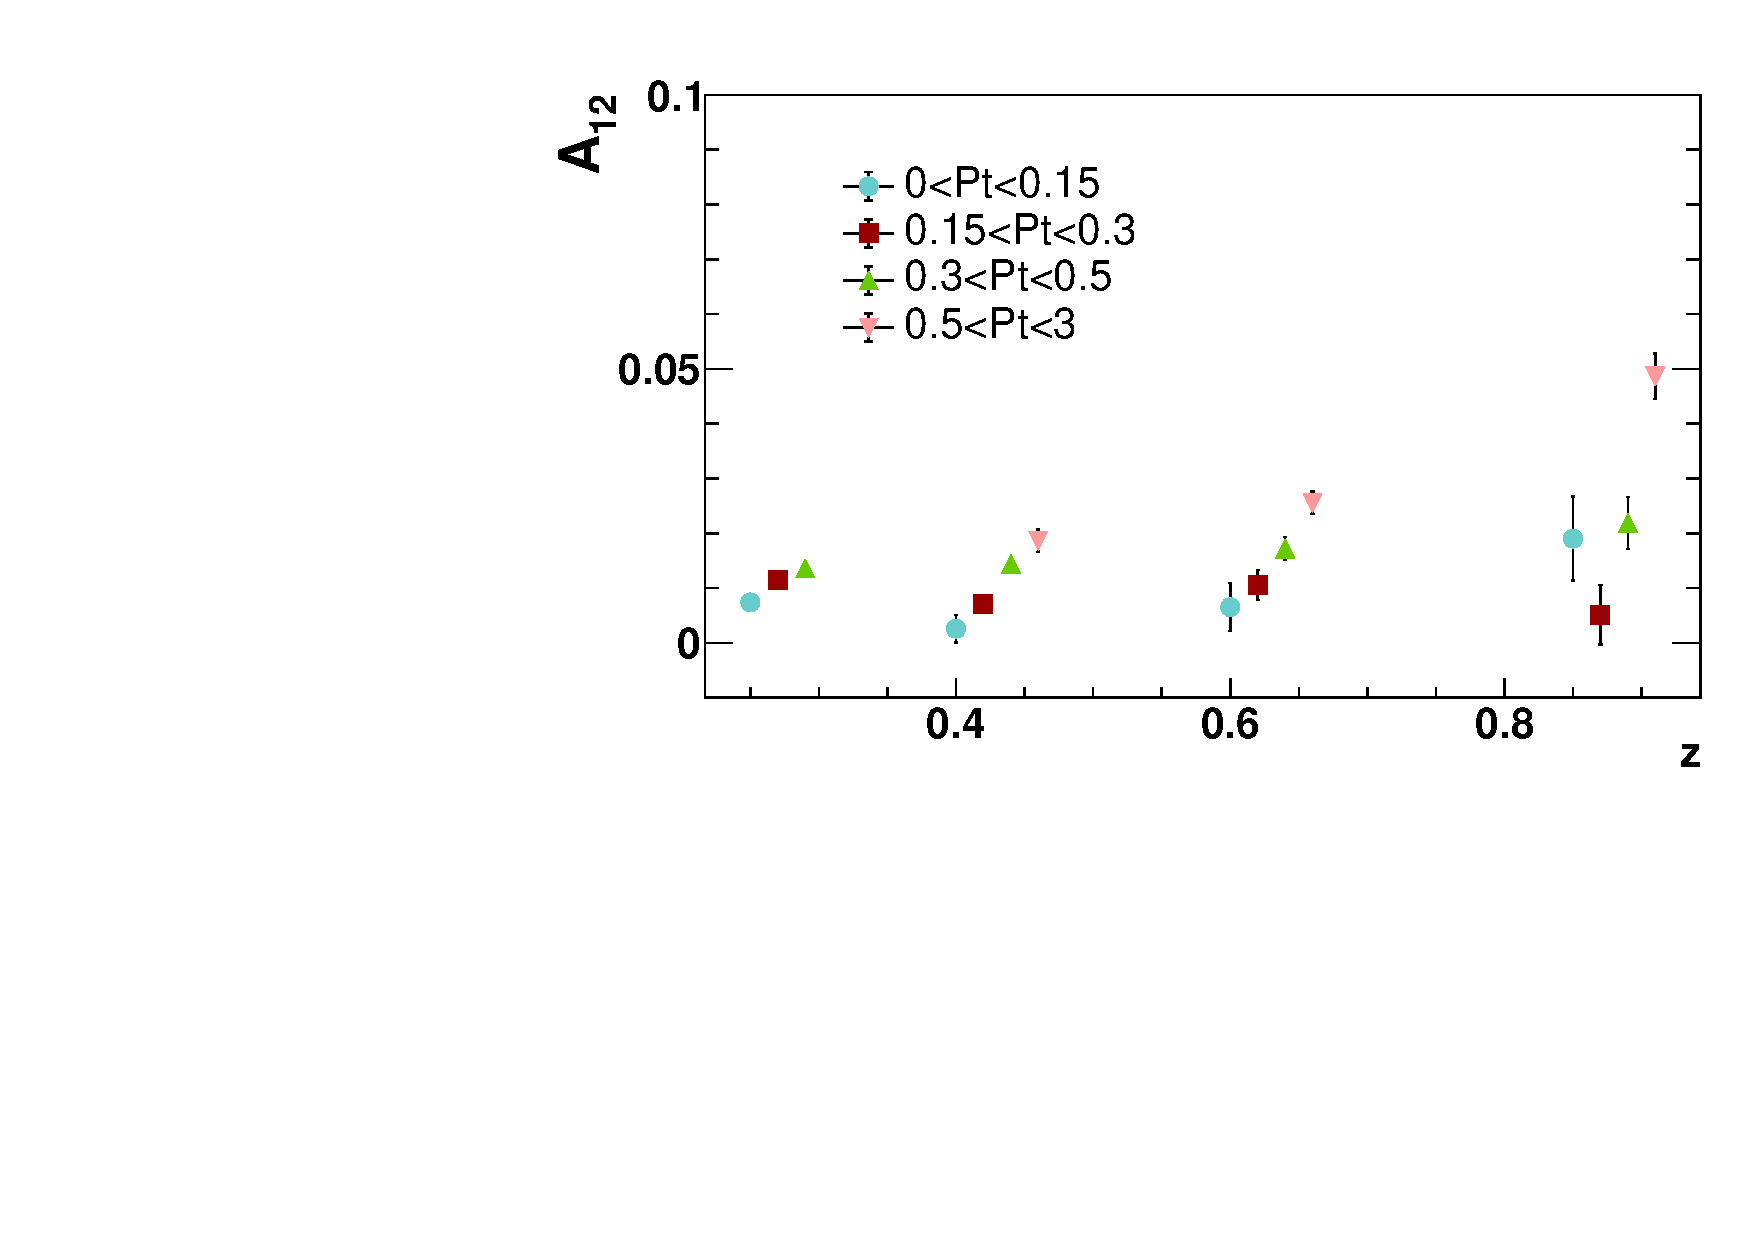
\includegraphics[width=60mm,natwidth=600,natheight=400]{figure_asy/Zpt.pdf}}
  \subfigure[With background correction (note that the uncertainties are inflated again)]{\label{fig:ptzbkgcorrection}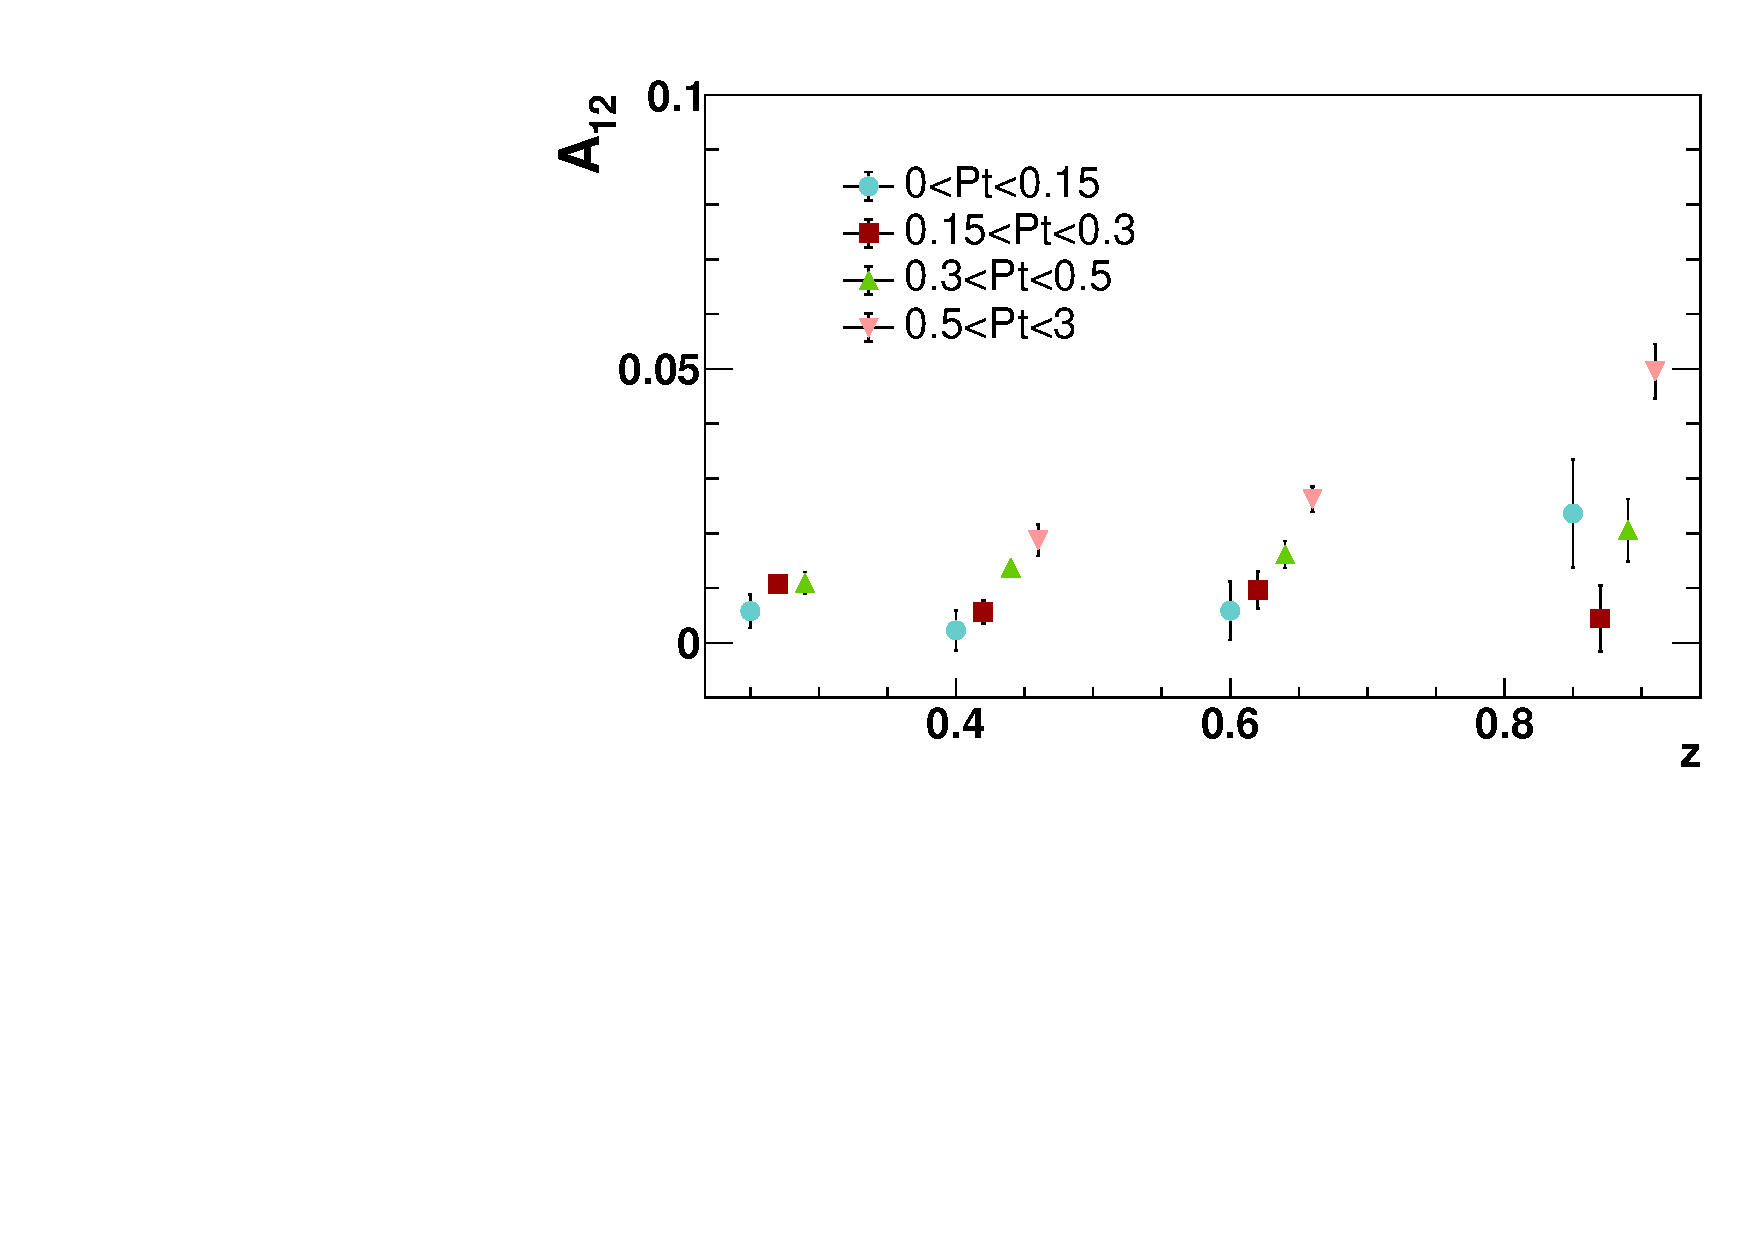
\includegraphics[width=60mm,natwidth=600,natheight=400]{figure_asy/Zpt_bkg_cor.pdf}}
  \subfigure[With background and thrust smearing correction]{\label{fig:ptzallcorrection}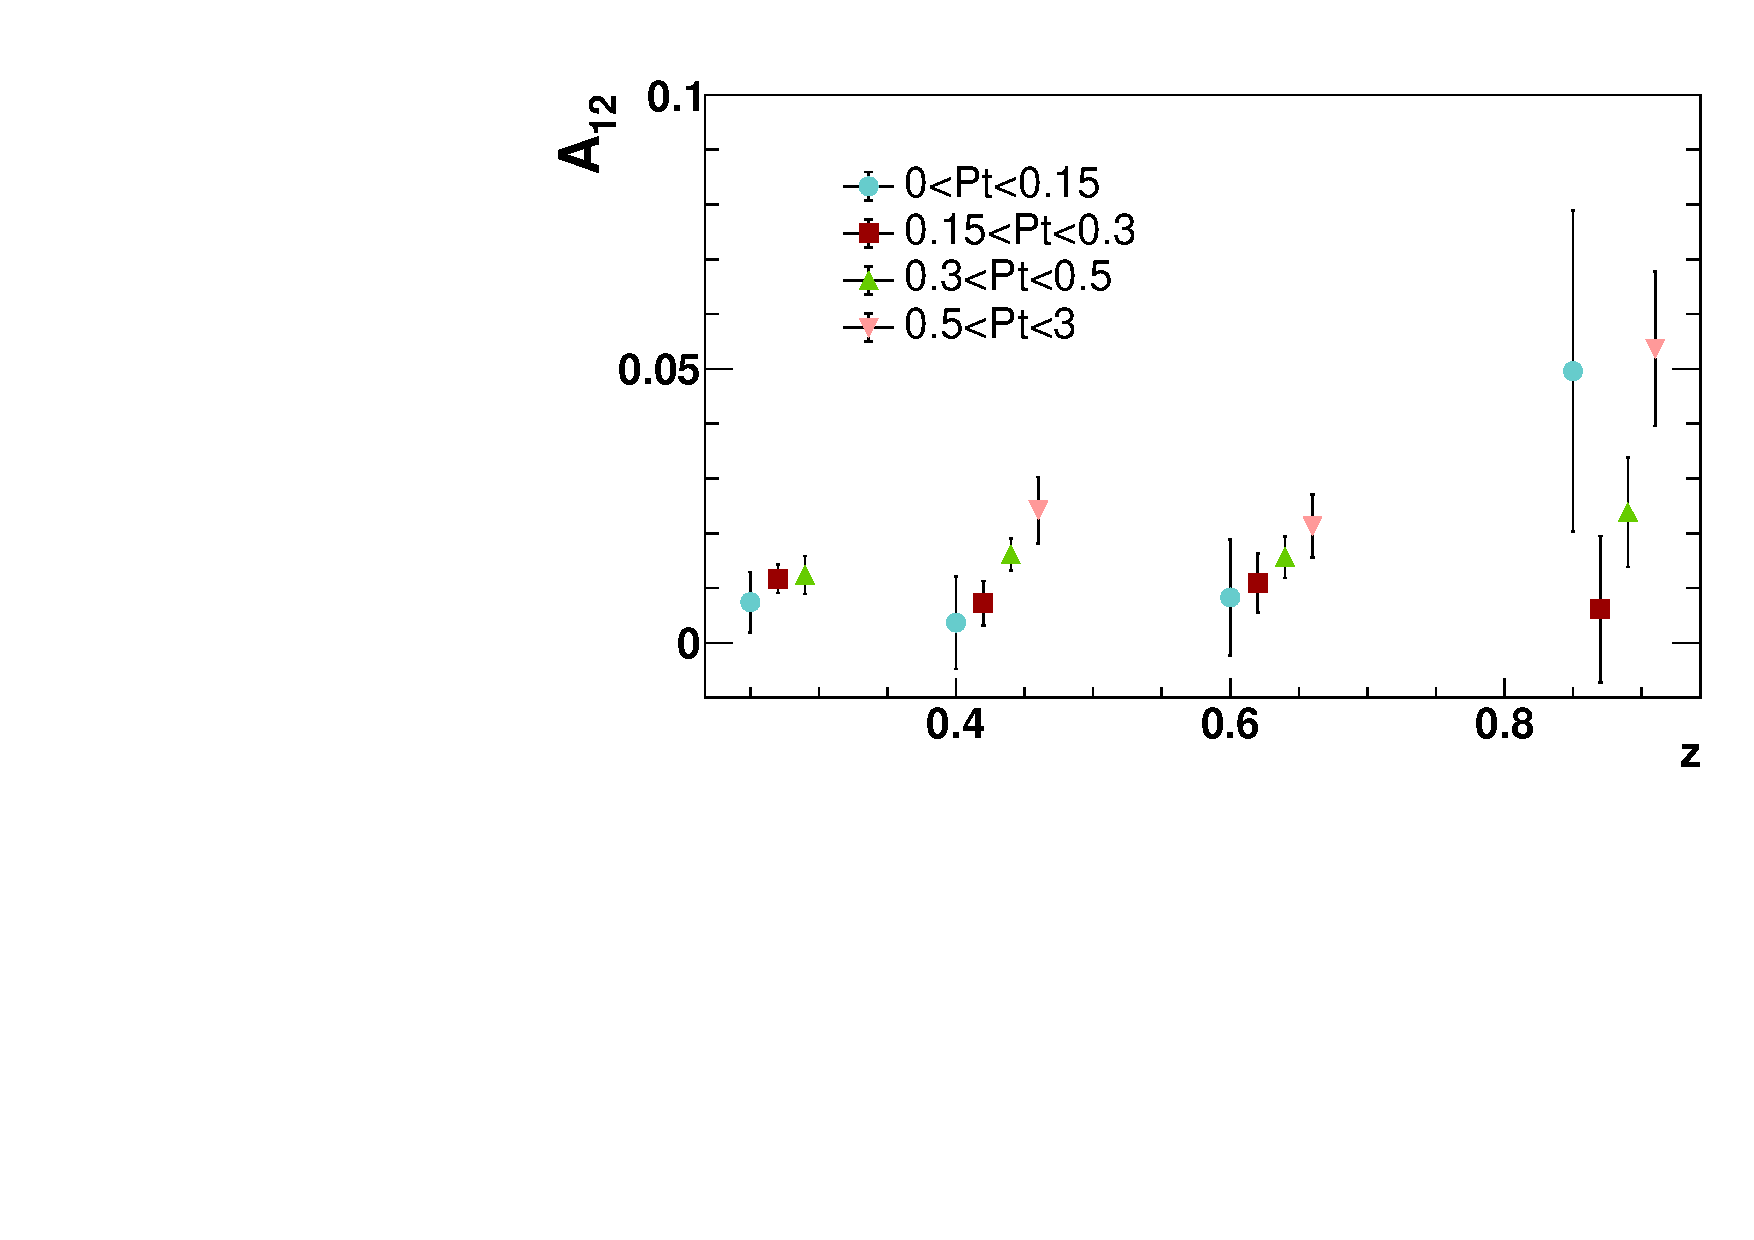
\includegraphics[width=60mm,natwidth=600,natheight=400]{figure_asy/Zpt_bkg&thrust_cor.pdf}}
\caption[$\pi^0$ double ratio after background and thrust-smearing corrections in $P_t$ vs.~$z$ bins]{$\pi^0$ double ratio in $P_t$ vs.~$z$ bins. The round points belong to the lowest $P_t$ bin, the red squares have $P_t$ range 0.15--0.3 GeV. The $P_t$ range for green triangles is 0.3--0.5~GeV and inverted pink triangles is 0.5-- 3.0~GeV. Each group of 4 points belongs to one $z$ bin as indicated on the x-axis. The range for the $z$ bins is $0.2<z_1<0.3$,  $0.3<z_1<0.5$, $0.5<z_1<0.7$ and $0.7<z_1<1$ from left to right. Notice that there are only 3 pink data points, because in the highest $P_t$ range no hadron pair falls in the $z$ range of 0.2--0.3.}
  \label{fig:ptzresult}
\end{figure}
